\documentclass{article}
\usepackage[utf8]{inputenc}
\usepackage{amsmath}
\usepackage{graphicx}
\title{Final Products for Hackathon}
%\author{howard.hao.ma }
%\date{November 2019}

\begin{document}

\maketitle

\section{Visualization for Publibike Dataset}
\subsection{Interactive visualization of number of rides per station at different hours in one day}
\begin{enumerate}
    \item The average number of rides per station of all dates (1 graph)
    \item The average number of rides per station of weekdays vs. weekends (2 graphs)
    \item The average number of rides per station of each day during a week (7 graphs)
\end{enumerate}

\subsection{Publibike vs. Swisscom Commuters}
\textbf{Data description:} 
\begin{itemize}
    \item Publibike: hourly data of number of rides; 
    \item Swisscom Data:hourly data of number of commuters
\end{itemize}
\subsubsection{Percentage of Publibike users among commuters}
\begin{align}
    y_i I_{-W} = \beta_1 + \beta_2 x_i I_{-W} + \varepsilon_i, \label{model1}
\end{align}
where $y_i$ represents the number of rides per hour, and $x_i$ represents the number of Swisscom commuters per hour.\\

% Table created by stargazer v.5.2.2 by Marek Hlavac, Harvard University. E-mail: hlavac at fas.harvard.edu
% Date and time: Sat, Nov 16, 2019 - 23:03:52
\begin{table}[!htbp] \centering 
  \caption{Model (\ref{model1})} 
  \label{} 
\begin{tabular}{@{\extracolsep{5pt}}lc} 
\\[-1.8ex]\hline 
\hline \\[-1.8ex] 
 & \multicolumn{1}{c}{\textit{Dependent variable:}} \\ 
\cline{2-2} 
\\[-1.8ex] & \# rides per hour\\ 
\# Swisscom commuters per hour & 0.005$^{***}$ \\ 
  & (0.001) \\ 
  & \\ 
 Constant & 24.172$^{***}$ \\ 
  & (1.070) \\ 
  & \\ 
\hline \\[-1.8ex] 
Observations & 768 \\ 
R$^{2}$ & 0.072 \\ 
Adjusted R$^{2}$ & 0.071 \\ 
Residual Std. Error & 18.833 (df = 766) \\ 
F Statistic & 59.793$^{***}$ (df = 1; 766) \\ 
\hline 
\hline \\[-1.8ex] 
\textit{Note:}  & \multicolumn{1}{r}{$^{*}$p$<$0.1; $^{**}$p$<$0.05; $^{***}$p$<$0.01} \\ 
\end{tabular} 
\end{table} 

\begin{figure}
    \centering
    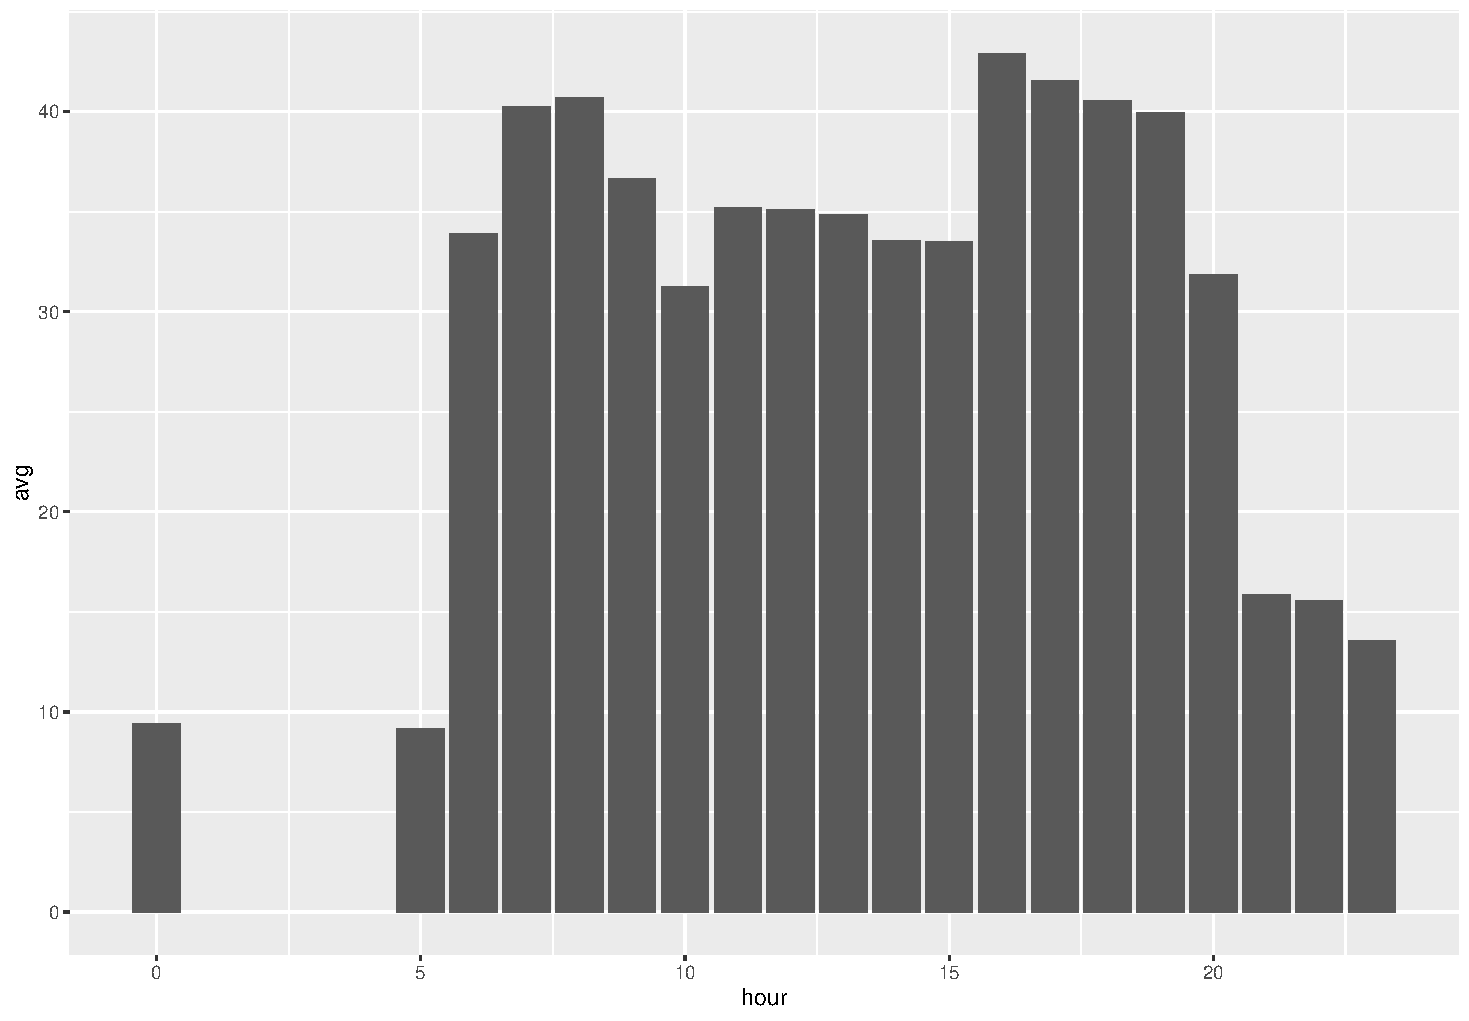
\includegraphics[width = \textwidth]{tpl_density.pdf}
    \caption{Histogram of number of Publibike rides by hour}
    \label{fig:my_label}
\end{figure}


\subsubsection{Substitution effect by buses}
\begin{align}
    y_i I_{-W} I_D = \beta_1 + \beta_2 x_i I_{-W} I_D + \varepsilon_i \label{model2} \\
    y_i I_{-W} I_E = \beta_1 + \beta_2 x_i I_{-W} I_E + \varepsilon_i \label{model3}\\
    y_i I_{-W} I_N = \beta_1 + \beta_2 x_i I_{-W} I_N + \varepsilon_i \label{model4}
\end{align}
where $I_D = 1$ represents day time $[6,19]$ when there are enough buses, $I_E = 1$ represents evening time $[20,23]$ when there are only a few buses and $I_N = 1$ represents night time $[0,5]$ when there is no bus.

% Table created by stargazer v.5.2.2 by Marek Hlavac, Harvard University. E-mail: hlavac at fas.harvard.edu
% Date and time: Sat, Nov 16, 2019 - 23:03:53
\begin{table}[!htbp] \centering 
  \caption{Model (\ref{model2})-(\ref{model4})} 
  \label{} 
\begin{tabular}{@{\extracolsep{5pt}}lccc} 
\\[-1.8ex]\hline 
\hline \\[-1.8ex] 
 & \multicolumn{3}{c}{\textit{Dependent variable:} \# rides per hour}\\ 
\cline{2-4} 
\\[-1.8ex] & 6am - 8pm & 9pm - 0am and 5am & 1am - 4am\\ 
\hline \\[-1.8ex] 
 \# Swisscom commuters & 0.003$^{***}$ & 0.088$^{***}$ & 0.113$^{**}$ \\ 
  & (0.001) & (0.013) & (0.043) \\ 
  & & & \\ 
 Constant & 28.600$^{***}$ & 7.525$^{**}$ & 3.666$^{*}$ \\ 
  & (1.657) & (3.729) & (2.150) \\ 
  & & & \\ 
\hline \\[-1.8ex] 
Observations & 521 & 174 & 73 \\ 
R$^{2}$ & 0.022 & 0.212 & 0.089 \\ 
Adjusted R$^{2}$ & 0.020 & 0.207 & 0.076 \\ 
Residual Std. Error & 16.594 (df = 519) & 21.521 (df = 172) & 8.434 (df = 71) \\ 
F Statistic & 11.759$^{***}$ (df = 1; 519) & 46.293$^{***}$ (df = 1; 172) & 6.902$^{**}$ (df = 1; 71) \\ 
\hline 
\hline \\[-1.8ex] 
\textit{Note:}  & \multicolumn{3}{r}{$^{*}$p$<$0.1; $^{**}$p$<$0.05; $^{***}$p$<$0.01} \\ 
\end{tabular} 
\end{table} 

\subsubsection{Control for number of buses on the road}
\begin{align}
    y_i I_{-W} = \beta_1 + \beta_2 x_i I_{-W} + \beta_3 z_i I_{-W} + \varepsilon_i,
\end{align}
where $z_i$ is the number of buses that are on the road.

% Table created by stargazer v.5.2.2 by Marek Hlavac, Harvard University. E-mail: hlavac at fas.harvard.edu
% Date and time: Sat, Nov 16, 2019 - 23:32:19
\begin{table}[!htbp] \centering 
  \caption{} 
  \label{} 
\begin{tabular}{@{\extracolsep{5pt}}lccc} 
\\[-1.8ex]\hline 
\hline \\[-1.8ex] 
 & \multicolumn{3}{c}{\textit{Dependent variable:}} \\ 
\cline{2-4} 
\\[-1.8ex] & \multicolumn{3}{c}{rides} \\ 
\\[-1.8ex] & (1) & (2) & (3)\\ 
\hline \\[-1.8ex] 
 commutes & $-$0.0004 & 0.001 & 0.077$^{***}$ \\ 
  & (0.001) & (0.001) & (0.020) \\ 
  & & & \\ 
 buses & 0.401$^{***}$ & 0.266$^{**}$ & 0.489 \\ 
  & (0.068) & (0.114) & (0.742) \\ 
  & & & \\ 
 Constant & 18.431$^{***}$ & 20.116$^{***}$ & 3.807 \\ 
  & (1.435) & (3.977) & (6.764) \\ 
  & & & \\ 
\hline \\[-1.8ex] 
Observations & 768 & 521 & 174 \\ 
R$^{2}$ & 0.112 & 0.032 & 0.214 \\ 
Adjusted R$^{2}$ & 0.110 & 0.029 & 0.205 \\ 
Residual Std. Error & 18.437 (df = 765) & 16.523 (df = 518) & 21.556 (df = 171) \\ 
F Statistic & 48.327$^{***}$ (df = 2; 765) & 8.680$^{***}$ (df = 2; 518) & 23.288$^{***}$ (df = 2; 171) \\ 
\hline 
\hline \\[-1.8ex] 
\textit{Note:}  & \multicolumn{3}{r}{$^{*}$p$<$0.1; $^{**}$p$<$0.05; $^{***}$p$<$0.01} \\ 
\end{tabular} 
\end{table} 

\end{document}
